\documentclass[12pt,a4paper,twoside]{book}
\usepackage{graphicx}
\usepackage{setspace}
\usepackage{natbib}
\usepackage[spanish]{babel}
\usepackage[utf8]{inputenc}
\usepackage{color}
\usepackage{hhline}
\usepackage{multirow}
\usepackage{subfigure}
\usepackage{acronym}
\usepackage{hyperref}
\usepackage{amsmath,amssymb}
\usepackage{fancyhdr}
\usepackage{epsfig, amsmath}
\usepackage{algorithm}
\usepackage{algorithmic}
\usepackage{longtable}

% configuraciones generales
\hypersetup{
linktocpage=true,
colorlinks=true,
linkcolor=blue,
citecolor=blue,
}
\definecolor{Hgray}{gray}{0.6}

\newenvironment{definition}[1][Definición]{\begin{trivlist}
\item[\hskip \labelsep {\bfseries #1}]}{\end{trivlist}}

\setlength{\topmargin}{0cm}
\setlength{\textheight}{23cm}
\setlength{\textwidth}{17cm}
\setlength{\oddsidemargin}{0cm}
\setlength{\evensidemargin}{0cm}
\setlength{\headheight}{1cm}

% indica que las 'sub-sub-secciones' están numeradas y aparecen en el índice
\setcounter{secnumdepth}{3}
\setcounter{tocdepth}{2}

% configuraciones para código
\renewcommand{\algorithmicrequire}{\textbf{Entrada:}}
\renewcommand{\algorithmicensure}{\textbf{Salida:}}

%%%%%%%%%%%%
% DOCUMENTO %
%%%%%%%%%%%%
\begin{document}

\setcounter{section}{0}
\renewcommand{\thesection}{\arabic{section}}

% portada
\begin{titlepage}
    \begin{center}

    \vspace*{0.5cm}

    
\includegraphics[width=0.6\textwidth]{figs/uoc_logo.png}

    \vspace{1cm}

    {\Huge \textbf{Propuesta de Trabajo Final de Máster}}

    \vspace{1.5cm}

    {\LARGE Sistema Multiagente para Verificación Automática de Hechos en Videos de YouTube}

    \vspace{0.5cm}

    {\Large Combatiendo la Desinformación mediante Procesamiento de Lenguaje Natural}

    \vspace{2cm}

    \textbf{Begoña Echavarren Sánchez}

    \vspace{0.5cm}

    \textit{Tutor: Josep-Anton Mir Tutusaus}

    \vspace{1.5cm}

    {\large Máster Universitario en Ciencia de Datos}

    {\large Universitat Oberta de Catalunya}

    \vspace{1cm}

    {\large PEC 1 - Definición del TFM}

    \vspace{0.5cm}

    {\large Octubre 2025}

    \end{center}
    \end{titlepage}

% copyright y ficha
\newpage
\thispagestyle{empty}

\pagenumbering{roman}
\setcounter{page}{1}
\pagestyle{plain}

\chapter*{Créditos/Copyright}

\vspace{1cm}

\begin{figure}[ht]
    \centering
    
\includegraphics[scale=1]{figs/license.png}
\end{figure}

Esta obra está sujeta a una licencia de Reconocimiento - NoComercial - SinObraDerivada 3.0 España de CreativeCommons.

\href{https://creativecommons.org/licenses/by-nc-nd/3.0/es/}{https://creativecommons.org/licenses/by-nc-nd/3.0/es/}

\vspace{1cm}

\chapter*{FICHA DEL TRABAJO FINAL}

\begin{table}[ht]
    \centering{}
    \renewcommand{\arraystretch}{2}
    \begin{tabular}{r | l}
        \hline
        Título del trabajo: & Sistema Multiagente para Verificación Automática\\
        & de Hechos en Videos de YouTube\\
        \hline
        Nombre del autor: & Begoña Echavarren Sánchez\\
        \hline
        Nombre del colaborador/a docente: & Josep-Anton Mir Tutusaus\\
        \hline
        Nombre del PRA: & [Nombre del PRA]\\
        \hline
        Fecha de entrega (mm/aaaa): & 10/2025\\
        \hline
        Titulación o programa: & Máster Universitario en Ciencia de Datos\\
        \hline
        Área del Trabajo Final: & Procesamiento de Lenguaje Natural\\
        & y Sistemas de Información\\
        \hline
        Idioma del trabajo: & Español\\
        \hline
        Palabras clave & fact-checking, NLP, multi-agent systems\\
        \hline
    \end{tabular}
\end{table}

% resumen
\thispagestyle{empty}

\section*{Resumen}

La desinformación en plataformas de video constituye un desafío creciente en la sociedad digital actual. Este trabajo propone el diseño, implementación y evaluación de un sistema end-to-end de verificación automática de hechos (fact-checking) para videos de YouTube, basado en una arquitectura multiagente que integra modelos de lenguaje de gran escala (LLMs), técnicas de procesamiento de lenguaje natural y recuperación de información en línea.

El sistema propuesto opera mediante un pipeline de cinco componentes principales: (1) extracción de transcripciones de video, (2) identificación automática de afirmaciones factuales mediante LLMs, (3) generación de consultas de búsqueda optimizadas, (4) recuperación y evaluación de evidencias desde fuentes web, y (5) síntesis de veredictos razonados con evaluación de confianza. Cada componente actúa como un agente especializado que procesa información estructurada mediante esquemas validados con Pydantic, garantizando robustez y trazabilidad en todo el proceso.

La implementación técnica combina Python 3.12 con frameworks modernos (Pydantic AI, FastAPI), modelos de lenguaje estado del arte (GPT-4o-mini) y alternativas de código abierto ejecutables localmente (Ollama Qwen 3), junto con técnicas de web scraping y evaluación de fiabilidad de fuentes. El proyecto incluye una interfaz web desarrollada en React con streaming en tiempo real mediante Server-Sent Events (SSE), proporcionando una experiencia de usuario interactiva durante el proceso de verificación.

Este trabajo aborda tanto aspectos de investigación en ciencia de datos (extracción de claims, evaluación de evidencias, detección de posturas) como de ingeniería de machine learning (arquitectura escalable, optimización de costes de LLMs, despliegue de sistemas productivos). Se plantea una evaluación del sistema mediante métricas cuantitativas de rendimiento y análisis cualitativo de casos de uso en diferentes temáticas de videos, con especial atención a contenido de economía, geopolítica y temas controversiales.

\vspace{1cm}

\noindent\textbf{Palabras clave:} fact-checking, natural language processing, large language models, information retrieval, multi-agent systems, misinformation detection, web scraping, automated verification, social media

\vspace{0.5cm}

\noindent\textbf{Área:} Procesamiento de Lenguaje Natural y Sistemas de Información

\noindent\textbf{Modalidad:} Trabajo ad hoc (a medida)

\newpage

\pagestyle{fancy}
\renewcommand{\chaptermark}[1]{ \markboth{#1}{}}
\renewcommand{\sectionmark}[1]{\markright{ \thesection.\ #1}}
\lhead[\fancyplain{}{\bfseries\thepage}]{\fancyplain{}{\bfseries\rightmark}}
\rhead[\fancyplain{}{\bfseries\leftmark}]{\fancyplain{}{\bfseries\thepage}}
\cfoot{}

% tabla de contenidos
\cleardoublepage
\phantomsection
\addcontentsline{toc}{chapter}{Índice}
\tableofcontents
% lista de figuras
\cleardoublepage
\phantomsection
\addcontentsline{toc}{chapter}{Lista de Figuras}
\listoffigures
% lista de tablas
\cleardoublepage
\phantomsection
\addcontentsline{toc}{chapter}{Lista de Tablas}
\listoftables

\thispagestyle{empty}

\pagenumbering{arabic}

\pagestyle{fancy}
\renewcommand{\chaptermark}[1]{ \markboth{#1}{}}
\renewcommand{\sectionmark}[1]{\markright{ \thesection.\ #1}}
\lhead[\fancyplain{}{\bfseries\thepage}]{\fancyplain{}{\bfseries\rightmark}}
\rhead[\fancyplain{}{\bfseries\leftmark}]{\fancyplain{}{\bfseries\thepage}}
\cfoot{}

\onehalfspacing

% capítulos del documento
\section{Introducción}

La desinformación en plataformas de video constituye un desafío creciente en la sociedad digital actual. YouTube, con más de 2 mil millones de usuarios activos mensuales, se ha convertido en una fuente primaria de información para millones de personas. Sin embargo, la ausencia de mecanismos efectivos de verificación de información permite la propagación de afirmaciones incorrectas o engañosas a escala masiva.

Este proyecto propone desarrollar un sistema automatizado end-to-end de verificación de hechos (fact-checking) para videos de YouTube, basado en una arquitectura multiagente que integra modelos de lenguaje de gran escala (LLMs), técnicas de procesamiento de lenguaje natural y recuperación de información en línea.

\begin{figure}[h]
\centering
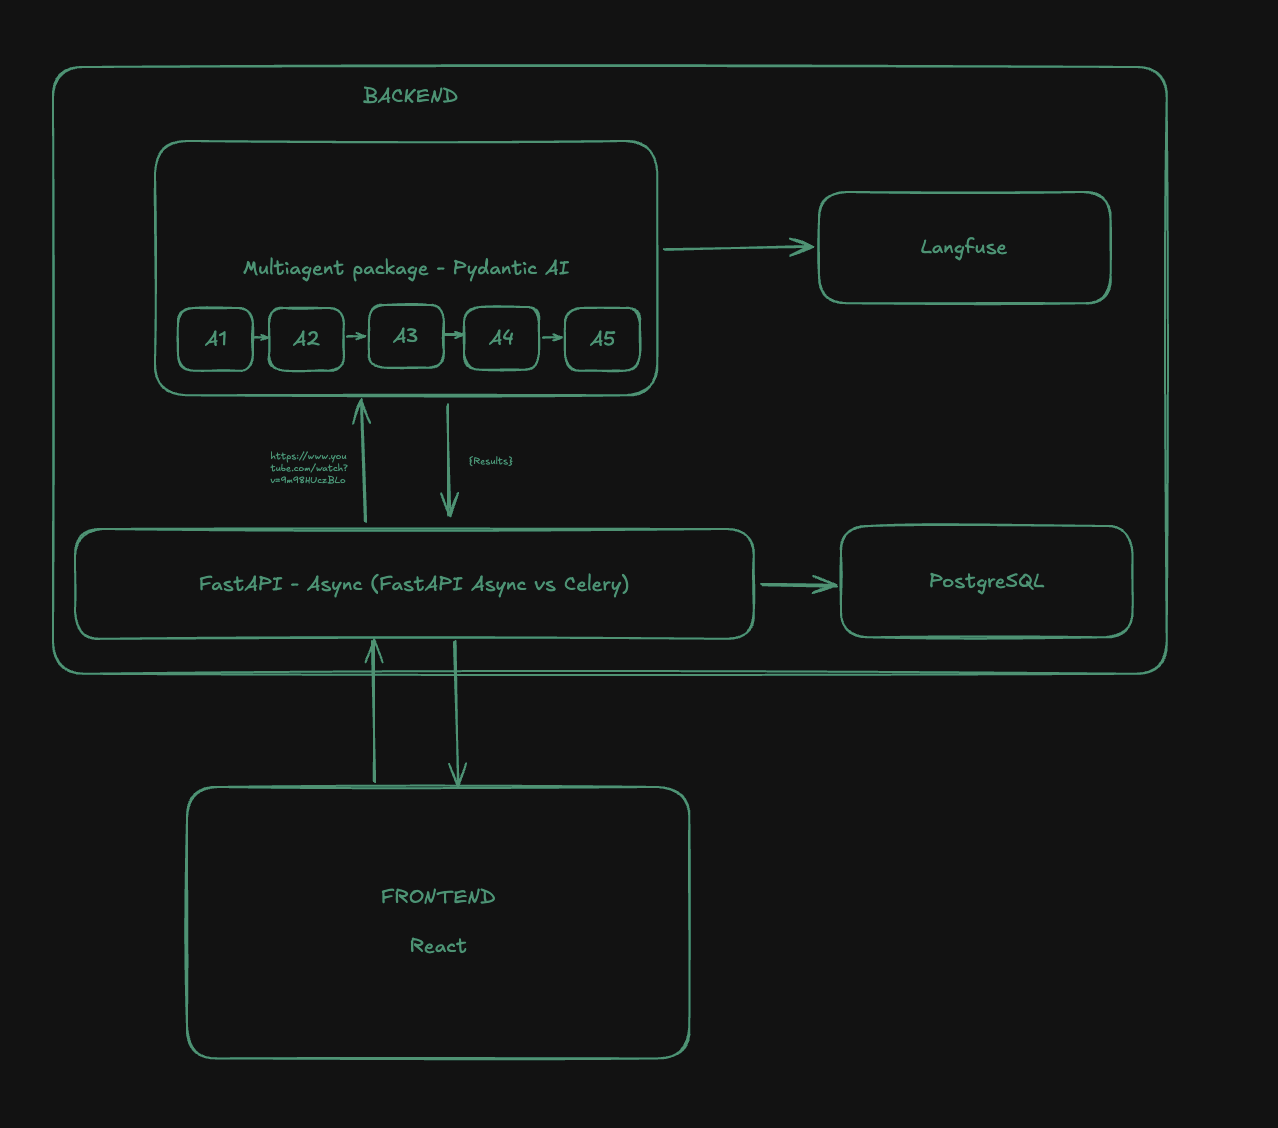
\includegraphics[width=0.85\textwidth]{./figs/system_architecture.png}
\caption{Arquitectura del sistema multiagente propuesto. Pipeline de cinco componentes especializados procesando secuencialmente desde transcripción hasta veredicto final.}
\label{fig:arquitectura}
\end{figure}

\subsection{Contexto y motivación}

\textbf{¿Cuál es el problema que necesita ser resuelto?}

El problema central es la falta de mecanismos automatizados y accesibles para verificar afirmaciones factuales en contenido audiovisual de plataformas digitales, específicamente videos de YouTube. Los usuarios individuales carecen de herramientas para verificar afirmaciones de forma sistemática, mientras que la verificación manual requiere habilidades avanzadas, tiempo considerable y recursos no siempre disponibles.

\textbf{¿Por qué es un tema relevante?}

\begin{itemize}
    \item \textbf{Impacto social:} La desinformación erosiona la confianza en instituciones, influye en decisiones políticas y afecta la salud pública.
    \item \textbf{Desafío tecnológico:} Integra múltiples áreas de investigación: procesamiento de lenguaje natural, recuperación de información, evaluación de credibilidad y razonamiento automático.
    \item \textbf{Escalabilidad necesaria:} El volumen de contenido generado diariamente (más de 500 horas de video por minuto en YouTube) hace inviable el fact-checking puramente humano.
    \item \textbf{Alfabetización mediática:} Herramientas que empoderan ciudadanos para evaluar críticamente información promueven pensamiento crítico.
\end{itemize}

\textbf{¿Cómo se está resolviendo el problema actualmente?}

Existen tres enfoques principales:

\begin{enumerate}
    \item \textbf{Fact-checking manual:} Organizaciones como Newtral, Maldita.es, FactCheck.org emplean periodistas especializados. Limitado por recursos humanos y temporal.
    \item \textbf{Sistemas académicos:} Proyectos como FEVER \citep{thorne2018fever}, FEVEROUS \citep{aly2021feverous}, ClaimBuster operan sobre bases de conocimiento estructuradas (Wikipedia) o requieren datasets curados. No están disponibles como productos.
    \item \textbf{APIs de verificación:} Google Fact Check Tools API agrega fact-checks publicados, pero solo cubre contenido ya verificado por profesionales.
\end{enumerate}

Ninguno de estos enfoques proporciona verificación automatizada end-to-end para contenido audiovisual generado continuamente por usuarios.

\textbf{¿Qué resultado se espera obtener?}

Este proyecto desarrollará un sistema funcional end-to-end que procese videos de YouTube mediante extracción de transcripciones, identifique afirmaciones factuales verificables, recupere evidencias desde múltiples fuentes web, evalúe la credibilidad de fuentes y postura de evidencias, y genere veredictos fundamentados con explicaciones transparentes mediante interfaz web accesible.

Adicionalmente, se realizará análisis comparativo de diferentes arquitecturas LLM (modelos comerciales vs. open-source), evaluación de trade-offs entre coste y rendimiento, y estudio de casos en diferentes dominios temáticos.

\textbf{Motivación personal:}

Mi interés en este proyecto surge de la confluencia de mi experiencia profesional como Machine Learning Engineer con más de 5 años en Data Science, mis intereses personales como consumidor de contenido educativo en YouTube sobre economía y geopolítica (donde frecuentemente encuentro afirmaciones que requieren verificación), y objetivos de desarrollo técnico. El proyecto combina aspectos de investigación y ingeniería que se alinean con mi visión profesional, mientras contribuye al bien social mediante una herramienta que fomenta el pensamiento crítico y alfabetización mediática.

\subsection{Objetivos}

\subsubsection{Objetivo Principal}

Diseñar, implementar y evaluar un sistema multiagente basado en modelos de lenguaje capaz de verificar automáticamente afirmaciones factuales en videos de YouTube mediante recuperación y análisis de evidencias web, generando veredictos fundamentados con estimación de confianza que sean útiles para usuarios finales.

\subsubsection{Objetivos Específicos}

\textbf{OE1. Diseño de arquitectura multiagente}
\begin{itemize}
    \item Definir pipeline de procesamiento con componentes especializados
    \item Establecer esquemas de datos estructurados para comunicación inter-agente
    \item Diseñar sistema de coordinación y flujo de información
\end{itemize}

\textbf{OE2. Implementación de componentes del sistema}
\begin{itemize}
    \item Desarrollar módulo de extracción de transcripciones desde YouTube
    \item Implementar agente de identificación de claims con clasificación de relevancia
    \item Crear generador de consultas de búsqueda optimizadas
    \item Desarrollar sistema de web scraping con evaluación de fiabilidad de fuentes
    \item Implementar generador de veredictos con razonamiento explicable
\end{itemize}

\textbf{OE3. Optimización de uso de LLMs}
\begin{itemize}
    \item Comparar rendimiento entre modelos comerciales (GPT-4o-mini) y open-source (Ollama Qwen 3)
    \item Analizar trade-offs entre coste, latencia y calidad de outputs
    \item Evaluar estrategias de optimización de prompts y structured outputs
\end{itemize}

\textbf{OE4. Evaluación del sistema}
\begin{itemize}
    \item Definir métricas de rendimiento técnico
    \item Establecer protocolos de evaluación cualitativa de veredictos
    \item Realizar estudios de caso en diferentes temáticas
    \item Analizar limitaciones y casos de fallo del sistema
\end{itemize}

\textbf{OE5. Implementación de sistema end-to-end}
\begin{itemize}
    \item Desarrollar API REST con streaming en tiempo real
    \item Crear interfaz web intuitiva para usuarios finales
    \item Garantizar reproducibilidad y documentación exhaustiva
\end{itemize}

\textbf{OE6. Análisis de implicaciones éticas}
\begin{itemize}
    \item Identificar sesgos potenciales en selección de fuentes
    \item Analizar riesgos de automatización de fact-checking
    \item Proponer salvaguardas y mejores prácticas
\end{itemize}

\subsubsection{Alcance del Proyecto}

\textbf{Incluye:} Videos de YouTube con transcripciones disponibles, afirmaciones factuales verificables mediante fuentes web públicas, contenido principalmente en inglés (con soporte experimental para español), procesamiento bajo demanda de videos individuales.

\textbf{No incluye:} Generación propia de transcripciones desde audio, verificación de contenido visual (imágenes, gráficos), sistema de caché o base de datos persistente, verificación en tiempo real o batch processing a gran escala, contenido de plataformas distintas a YouTube.

\subsection{Sostenibilidad, diversidad y desafíos ético/sociales}

Esta sección evalúa el impacto del proyecto en las tres dimensiones de la Competencia de Compromiso Ético y Global (CCEG) establecida por la UOC.

\begin{description}
    \item[Sostenibilidad] El uso de modelos de lenguaje de gran escala implica un consumo energético significativo durante la inferencia. Este proyecto considera explícitamente el impacto ambiental mediante evaluación de alternativas eficientes (comparación entre modelos comerciales cloud y modelos open-source ejecutables localmente), análisis de trade-offs documentando consumo de recursos (tokens procesados, tiempo de ejecución, coste económico), y optimización de prompts para minimizar tokens procesados sin sacrificar calidad.

    Durante el desarrollo se priorizarán modelos locales durante experimentación, implementación de mecanismos de control de uso, y documentación transparente del consumo de recursos. En las conclusiones se incluirá análisis crítico sobre sostenibilidad del sistema a escala, discutiendo si la automatización justifica el consumo energético frente a beneficios sociales.

    El proyecto se relaciona con los Objetivos de Desarrollo Sostenible (ODS): \textbf{ODS 4 (Educación de Calidad)} como herramienta de alfabetización mediática, \textbf{ODS 16 (Paz, Justicia e Instituciones Sólidas)} combatiendo desinformación, y \textbf{ODS 10 (Reducción de Desigualdades)} democratizando acceso a verificación.

    \item[Comportamiento ético y responsabilidad social] El proyecto tiene múltiples impactos éticos identificados:

    (1) \textbf{Automatización y empleo:} El sistema podría percibirse como amenaza para verificadores profesionales. Se posiciona como herramienta de apoyo que automatiza pasos preliminares, permitiendo a profesionales enfocarse en análisis complejos.

    (2) \textbf{Sesgo algorítmico:} Los LLMs pueden perpetuar sesgos presentes en datos de entrenamiento. El proyecto implementa transparencia total en fuentes consultadas, presentación de evidencias con diferentes posturas, evaluación explícita de confianza en veredictos, y advertencias sobre limitaciones.

    (3) \textbf{Riesgo de amplificación:} Al citar afirmaciones incorrectas durante verificación, existe riesgo de amplificar desinformación. Mitigación mediante presentación siempre contextualizada con veredicto, no indexación pública de claims individuales, y enfoque en proceso educativo.

    (4) \textbf{Privacidad:} El proyecto respeta políticas de YouTube y no procesa contenido privado ni viola términos de uso.

    Como profesional de Data Science, este proyecto se adhiere a principios deontológicos de transparencia, no maleficencia, beneficencia social y responsabilidad.

    \item[Diversidad, género y derechos humanos] La interfaz web se diseñará siguiendo principios de accesibilidad (contraste de colores WCAG 2.1, navegación por teclado, textos alternativos, diseño responsive).

    Se reconoce limitación en diversidad lingüística: modelos LLM tienen mejor rendimiento en inglés. Mitigación mediante soporte experimental para español y documentación de limitaciones lingüísticas. Las fuentes web indexadas pueden tener sesgo geográfico/cultural; el sistema evaluará diversidad de perspectivas cuando disponible.

    El proyecto evita enfocarse exclusivamente en temáticas asociadas a demografías específicas, seleccionando casos de prueba diversos. Respecto a derechos fundamentales: impacto positivo en derecho a la información, respeto a libertad de expresión (no censura, solo proporciona contexto), y protección de privacidad (no procesa datos personales).
\end{description}

\subsection{Enfoque y metodología}

\subsubsection{Estrategia de Investigación}

Este proyecto adopta una metodología de \textbf{Investigación y Desarrollo} (Design Science Research), combinando investigación en ciencia de datos con ingeniería de software aplicada. Esta estrategia es apropiada porque: (1) el problema es complejo y multidisciplinar requiriendo integración de NLP, recuperación de información y diseño de sistemas; (2) el resultado debe ser sistema operativo, no solo análisis teórico; (3) las decisiones técnicas se validan mediante experimentación empírica; (4) el desarrollo modular permite mejoras incrementales basadas en evaluación continua.

\textbf{Estrategias alternativas consideradas y descartadas:}

\begin{itemize}
    \item \textbf{Investigación puramente teórica:} Análisis conceptual sin implementación. Descartada porque no permite validación empírica ni produce herramienta utilizable.
    \item \textbf{Adaptación de solución existente:} Extensión de sistemas como HySonLab/FactAgent \citep{hysonlab2025factagent}. Descartada porque limita aprendizaje y reduce originalidad.
    \item \textbf{Enfoque solo en un componente:} Profundizar exclusivamente en extracción de claims. Descartada porque no aborda problema E2E ni tiene impacto práctico significativo.
\end{itemize}

\textbf{Estrategia seleccionada:} Desarrollo E2E con evaluación comparativa. Combina implementación completa del pipeline (valor ingenieril), experimentación con diferentes modelos (valor investigativo), evaluación cuantitativa y cualitativa (rigor científico), e interfaz funcional (aplicabilidad real).

\subsubsection{Metodología de Desarrollo}

El sistema sigue arquitectura de pipeline (Figura \ref{fig:arquitectura}) con cinco agentes especializados:

\begin{enumerate}
    \item \textbf{Transcriptor:} Extrae texto desde videos de YouTube
    \item \textbf{Claim Extractor:} Identifica afirmaciones factuales verificables
    \item \textbf{Query Generator:} Crea consultas de búsqueda optimizadas
    \item \textbf{Online Search:} Recupera y evalúa evidencias web
    \item \textbf{Output Generator:} Sintetiza veredictos fundamentados
\end{enumerate}

Cada componente opera sobre esquemas de datos estructurados definidos con Pydantic, garantizando validación de tipos y contratos claros entre módulos.

\textbf{Proceso de desarrollo iterativo modular:}
\begin{enumerate}
    \item Implementación básica de cada componente
    \item Integración E2E del pipeline completo ("MVP")
    \item Refinamiento iterativo módulo por módulo
    \item Evaluación comparativa con diferentes configuraciones
\end{enumerate}

\subsubsection{Técnicas y Herramientas}

\textbf{Procesamiento de Lenguaje Natural:} Prompting avanzado con LLMs (chain-of-thought, few-shot), structured outputs mediante Pydantic, análisis de stance (apoya/refuta/mixto).

\textbf{Recuperación de Información:} Web scraping con Selenium, evaluación de credibilidad (análisis WHOIS, características de sitio), estrategias de búsqueda diversificadas.

\textbf{Stack Tecnológico:}
\begin{itemize}
    \item \textbf{Backend:} Python 3.12, Pydantic AI, FastAPI, Uvicorn
    \item \textbf{LLMs:} OpenAI GPT-4o-mini, Ollama Qwen 3 (1.7B/4B/8B)
    \item \textbf{Frontend:} React 18.3, Vite, Tailwind CSS
    \item \textbf{Herramientas:} uv (gestión dependencias), ruff (linting), mypy (type checking)
\end{itemize}

\textbf{Evaluación:}

Métricas cuantitativas: tiempo de procesamiento por video, coste por verificación (tokens consumidos), número de fuentes recuperadas por claim, distribución de stances (evidencias a favor/contra).

Evaluación cualitativa: revisión manual de relevancia de claims extraídos, análisis de coherencia de veredictos, comparación con fact-checks profesionales cuando disponibles.

\subsection{Planificación}

\subsubsection{Cronograma General}

El proyecto se desarrolla durante el semestre académico 2025-2026, alineado con entregas de PECs (Tabla \ref{tab:cronograma}).

\begin{table}[h]
\centering
\begin{tabular}{|l|l|l|l|}
\hline
\textbf{Fase} & \textbf{Periodo} & \textbf{Entregable} & \textbf{Fecha límite} \\
\hline
PEC 1 & Sep-Oct 2025 & Definición TFM & 12 octubre 2025 \\
PEC 2 & Oct-Nov 2025 & Seguimiento 1 & 16 noviembre 2025 \\
PEC 3 & Nov-Dic 2025 & Seguimiento 2 & 21 diciembre 2025 \\
PEC 4 & Ene 2026 & Seguimiento final & 18 enero 2026 \\
Memoria & Ene-Feb 2026 & Documento completo & 8 febrero 2026 \\
Defensa & Feb 2026 & Presentación & Por determinar \\
\hline
\end{tabular}
\caption{Cronograma general del proyecto}
\label{tab:cronograma}
\end{table}

\begin{figure}[h]
\centering
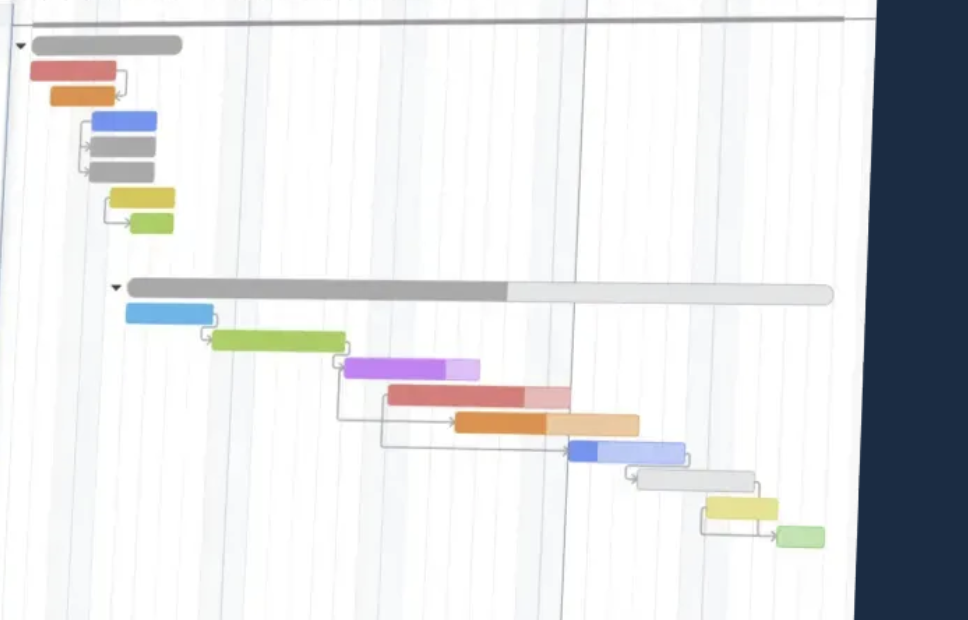
\includegraphics[width=\textwidth]{./figs/gantt_diagram.png}
\caption{Diagrama de Gantt mostrando la planificación temporal de todas las fases del proyecto con hitos de entrega de PECs.}
\label{fig:gantt}
\end{figure}

\subsubsection{Descripción de Fases}

\textbf{Fase 1: Investigación y Diseño (Sep 25 - Oct 15, 2025) - 3 semanas}

Actividades: Revisión de literatura (fact-checking, sistemas multiagente, LLMs), diseño detallado de arquitectura (componentes, esquemas, flujo), selección de tecnologías y modelos, elaboración de PEC 1.

Hitos: Documento de arquitectura completado, stack tecnológico definido, PEC 1 entregada.

\textbf{Fase 2: Implementación Core (Oct 16 - Nov 15, 2025) - 4 semanas}

Actividades: Setup inicial del proyecto, implementación secuencial de los cinco componentes (Transcriptor 3 días, Claim Extractor 5 días, Query Generator 4 días, Online Search 7 días, Output Generator 5 días), integración pipeline E2E con logging (3 días), elaboración de PEC 2.

Hitos: MVP funcional end-to-end operativo, todos los componentes implementados, PEC 2 entregada.

\textbf{Fase 3: Optimización y Evaluación (Nov 16 - Dic 21, 2025) - 5 semanas}

Actividades: Experimentación con optimización de prompts (1 semana), comparación GPT-4o-mini vs Ollama Qwen 3 con análisis trade-offs (1.5 semanas), evaluación en 15-20 videos diversos con documentación (1 semana), medición de métricas (3 días), implementación de mejoras (1 semana), elaboración de PEC 3.

Hitos: Evaluación cuantitativa completada, análisis comparativo de modelos realizado, PEC 3 entregada.

\textbf{Fase 4: Interfaz y Deployment (Dic 22, 2025 - Ene 18, 2026) - 4 semanas}

Actividades: Desarrollo API REST con FastAPI y Server-Sent Events (1 semana), frontend React con componentes UI e integración SSE (1.5 semanas), testing e integración (3 días), documentación técnica (README, guías, API docs - 2 días), elaboración de PEC 4.

Hitos: Sistema E2E con UI funcional, documentación técnica completa, PEC 4 entregada.

\textbf{Fase 5: Memoria y Análisis Final (Ene 19 - Feb 8, 2026) - 3 semanas}

Actividades: Redacción de memoria completa (2 semanas), análisis de implicaciones éticas (2 días), trabajo futuro (1 día), revisión y correcciones (3 días), preparación de presentación (2 días).

Hitos: Memoria final entregada, presentación preparada.

\subsubsection{Recursos Necesarios}

\textbf{Hardware:} Ordenador personal con 16GB RAM mínimo para ejecutar Ollama, acceso a internet estable.

\textbf{Software:} Python 3.12 y librerías (open-source), Ollama (gratuito), VS Code (gratuito), LaTeX (gratuito).

\textbf{Servicios externos:} API de OpenAI (presupuesto personal €50-100), hosting opcional (AWS/Vercel ~€20/mes, no crítico).

\textbf{Tiempo:} Dedicación estimada 15-20 horas/semana durante 5 meses, total aproximado 300-400 horas.

\subsubsection{Gestión de Riesgos}

La Tabla \ref{tab:riesgos} presenta los principales riesgos identificados con sus estrategias de mitigación.

\begin{table}[h]
\centering
\small
\begin{tabular}{|p{4cm}|c|c|p{5cm}|}
\hline
\textbf{Riesgo} & \textbf{Prob.} & \textbf{Impacto} & \textbf{Mitigación} \\
\hline
Costes API OpenAI excesivos & Media & Alto & Usar Ollama en desarrollo; establecer límites de gasto \\
\hline
Rendimiento modelos locales insuficiente & Media & Medio & GPT-4o-mini como fallback; optimizar prompts \\
\hline
Web scraping bloqueado por sitios & Alta & Medio & Rate limiting; rotar user agents; fuentes alternativas \\
\hline
Tiempos procesamiento muy largos & Media & Medio & Optimizar pipeline; procesamiento paralelo de claims \\
\hline
Calidad transcripciones YouTube baja & Baja & Medio & Filtrar por calidad; priorizar subtítulos manuales \\
\hline
\end{tabular}
\caption{Análisis de riesgos y estrategias de mitigación}
\label{tab:riesgos}
\end{table}

Estrategias de contingencia: desarrollo modular permite ajustar alcance, versiones incrementales garantizan entregable funcional, documentación continua evita pérdidas de información, evaluación temprana detecta problemas antes de entrega final.

\subsection{Resumen de los productos del proyecto}

Este TFM generará los siguientes productos:

\begin{enumerate}
    \item \textbf{Sistema de fact-checking automatizado:} Pipeline E2E funcional con cinco componentes modulares implementados en Python 3.12.
    \item \textbf{API REST con streaming:} Servicio FastAPI con actualizaciones en tiempo real vía Server-Sent Events.
    \item \textbf{Interfaz web:} Aplicación React responsive que permite ingresar URLs de YouTube y visualizar resultados intuitivamente.
    \item \textbf{Análisis comparativo de modelos LLM:} Evaluación empírica de rendimiento, coste y calidad entre GPT-4o-mini y Ollama Qwen 3.
    \item \textbf{Conjunto de evaluación:} Dataset de 15-20 videos procesados con análisis cualitativo y métricas documentadas.
    \item \textbf{Documentación técnica:} Repositorio de código con README, guías de instalación, documentación de API y ejemplos.
    \item \textbf{Memoria del TFM:} Documento académico completo.
\end{enumerate}

Los productos técnicos estarán disponibles en repositorio público de GitHub. La memoria seguirá estándares académicos de la UOC y podrá publicarse en repositorio institucional O2.

\subsection{Breve descripción de los demás capítulos del informe}

\textit{Nota: Esta sección describe la estructura prevista para la memoria final del TFM.}

\textbf{Capítulo 2: Estado del Arte} - Revisión exhaustiva de literatura sobre fact-checking automático, sistemas multiagente con LLMs, técnicas de NLP aplicadas a verificación, y posicionamiento de esta propuesta.

\textbf{Capítulo 3: Metodología y Diseño} - Descripción detallada de arquitectura del sistema, decisiones de diseño por componente, esquemas de datos Pydantic, estrategias de prompting.

\textbf{Capítulo 4: Implementación} - Detalles de implementación de cada módulo, integración entre componentes, manejo de errores, optimizaciones.

\textbf{Capítulo 5: Evaluación y Resultados} - Métricas cuantitativas, análisis cualitativo de casos de prueba, comparación de modelos LLM, discusión de limitaciones.

\textbf{Capítulo 6: Análisis Ético} - Profundización en implicaciones éticas, sesgos, riesgos, salvaguardas y recomendaciones.

\textbf{Capítulo 7: Conclusiones y Trabajo Futuro} - Síntesis de logros, evaluación crítica de objetivos, lecciones aprendidas, limitaciones y extensiones futuras.

\textbf{Anexos} - Código relevante, ejemplos de outputs, documentación API, material complementario.

\section{Glosario}

\begin{description}
    \item[API (Application Programming Interface)] Interfaz que permite la comunicación entre diferentes componentes de software.
    \item[Claim] Afirmación factual susceptible de ser verificada mediante evidencias.
    \item[E2E (End-to-End)] Sistema completo desde entrada hasta salida, sin componentes intermedios externos.
    \item[Fact-checking] Proceso de verificación de hechos mediante consulta de fuentes fiables.
    \item[FastAPI] Framework web moderno para Python orientado a construcción de APIs REST.
    \item[LLM (Large Language Model)] Modelo de lenguaje de gran escala entrenado con grandes cantidades de texto.
    \item[NLP (Natural Language Processing)] Procesamiento de Lenguaje Natural, campo de IA que estudia interacción entre computadoras y lenguaje humano.
    \item[Ollama] Herramienta para ejecutar modelos de lenguaje open-source localmente.
    \item[Pipeline] Secuencia de componentes de procesamiento donde output de uno es input del siguiente.
    \item[Pydantic] Librería Python para validación de datos usando type hints.
    \item[SSE (Server-Sent Events)] Tecnología que permite servidor enviar actualizaciones automáticas a clientes web.
    \item[Stance] Postura de una evidencia respecto a una afirmación (apoya/refuta/mixta/no clara).
    \item[Web scraping] Técnica de extracción automatizada de datos desde páginas web.
\end{description}

% bibliografía
\addcontentsline{toc}{chapter}{Bibliografía}
\bibliographystyle{plain}
\bibliography{references}

\end{document}
